\documentclass{article}
\usepackage{pslatex}
\usepackage{amssymb}
\pagestyle{empty}
\usepackage{graphicx}
\usepackage{grffile}
\usepackage{fullpage}
\begin{document}
\section{Morphology: phasedataCH.0004 }
\begin{small}
\begin{center}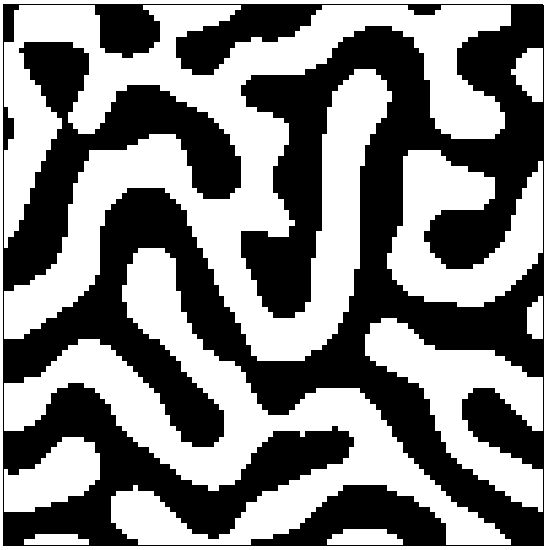
\includegraphics[width=0.2\textwidth]{/home/owodo/MINE/PROJECTS/GraSPI/GraSPI-2.0/examples/101x101/phi0_0.5/figs/phasedataCH.0004.plt.jpg} \end{center}
ETA ABS |  Weighted fraction of polymer vertices: 0.497402\\
STATS |  Number of polymer CCs: 10\\
STATS |  Number of fullerene CCs 9\\
STATS |  Number of polymer CCs conn to anode: 5\\
STATS |  Number of fullerene CCs conn to cathode: 3\\
STATS |  Number of vertices: 10201\\
STATS |  Number of polymer vertices: 5074\\
STATS |  Number of fullerene vertices: 5127\\
ETA ABS |  Fraction of polymer vertices: 0.497402\\
ETA CT |  Fraction of useful vertices - w/o islands: 0.468385\\
ETA CT |  Fraction of polymer vertices conn to anode: 0.662791\\
ETA CT |  Fraction of fullerene vertices conn to cathode: 0.27599\\
ETA DISS |  Weighted fraction of polymer vertices in 10 distance to interface: 0.797328\\
ETA DISS |  Number of interface 1st order edges: 1842\\
STATS |  Number of int edges with complementary paths: 262\\
ETA CT |  Fraction of interface with complementary paths to cathode and anode: 0.142237\\
STATS |  Number of polymer int vertices with path to anode: 1188\\
STATS |  Number of fullerene int vertices with path to cathode: 552\\
ETA CT |  Fraction of polymer vertices with straight rising paths (t=1): 0.0779066\\
ETA CT |  Fraction of fullerene vertices with straight rising paths (t=1): 0.15689\\
\\
 time check:\\
Reading done: +0.202552s\\
CC determined: +0.0674751s\\
ALL performance indicators computed: +0.213367s\\
----------------\\
total: 0.483407s\\

\end{small}
\begin{center}
\parbox{0.33\textwidth}{\begin{scriptsize}Distance from Fullerene Vertex to Cathode\end{scriptsize}\newline
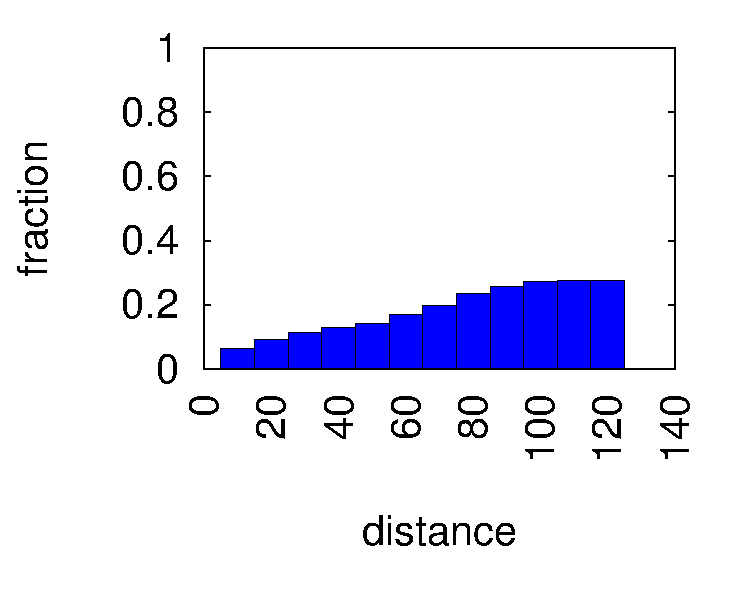
\includegraphics[width=0.3\textwidth]{/home/owodo/MINE/PROJECTS/GraSPI/GraSPI-2.0/examples/101x101/phi0_0.5/histograms/phasedataCH.0004.txtCumHistogramFullereneToCathode.pdf}} 
\parbox{0.33\textwidth}{\begin{scriptsize}Distance from Polymer Vertex to Anode\end{scriptsize}\newline
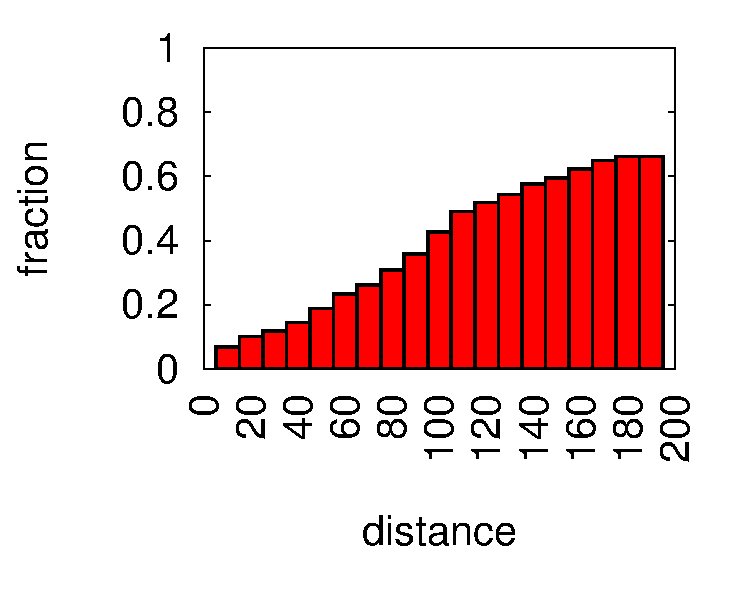
\includegraphics[width=0.3\textwidth]{/home/owodo/MINE/PROJECTS/GraSPI/GraSPI-2.0/examples/101x101/phi0_0.5/histograms/phasedataCH.0004.txtCumHistogramPolymerToAnode.pdf}}
\parbox{0.33\textwidth}{\begin{scriptsize}Distance from Polymer Vertex to Interface\end{scriptsize}\newline
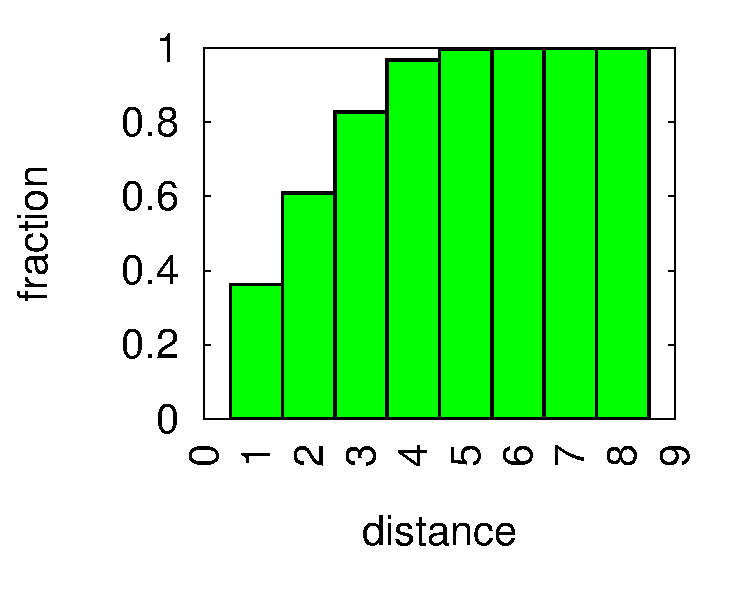
\includegraphics[width=0.3\textwidth]{/home/owodo/MINE/PROJECTS/GraSPI/GraSPI-2.0/examples/101x101/phi0_0.5/histograms/phasedataCH.0004.txtCumHistogramPolymerToInterface.pdf}} \newline
\parbox{0.49\textwidth}{\begin{scriptsize}Distance from Interface to Cathode via Fullerene vertices \end{scriptsize}\newline
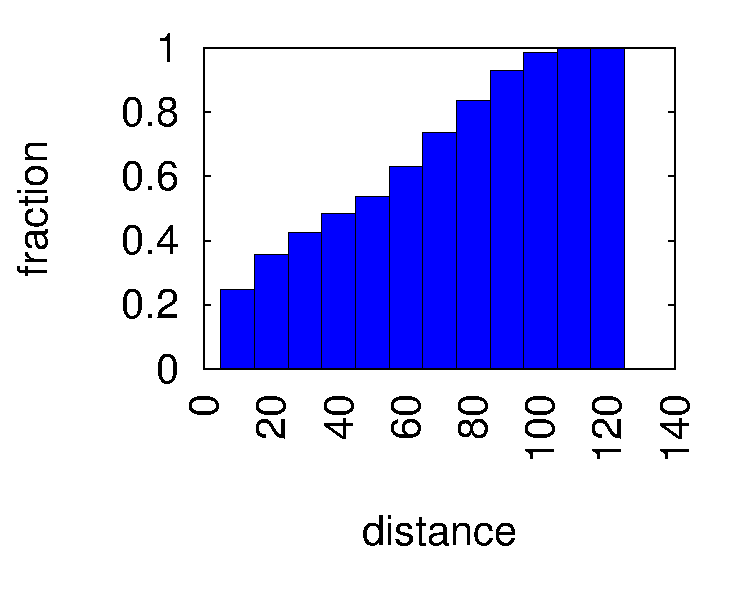
\includegraphics[width=0.33\textwidth]{/home/owodo/MINE/PROJECTS/GraSPI/GraSPI-2.0/examples/101x101/phi0_0.5/histograms/phasedataCH.0004.txtCumHistogramInterfaceToCathodeViaFullerene.pdf}}
\parbox{0.49\textwidth}{\begin{scriptsize}Distance from Interface to Anode via Polymer vertices \end{scriptsize}\newline
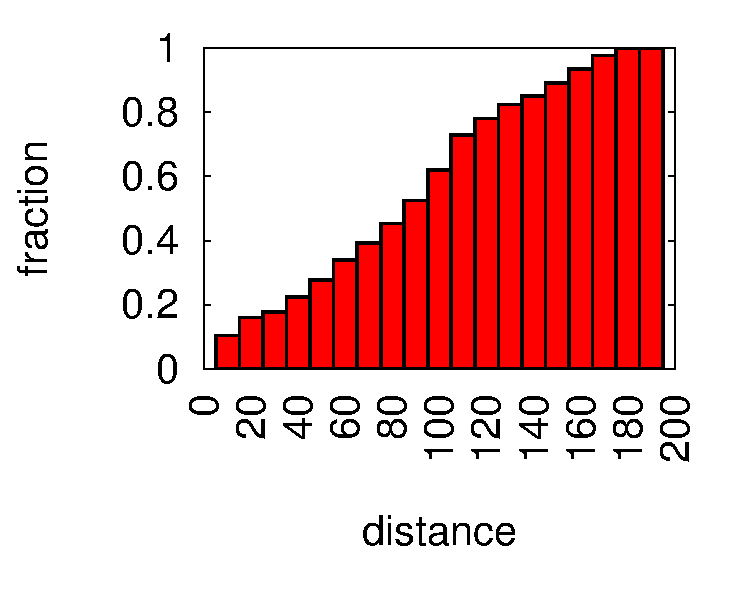
\includegraphics[width=0.33\textwidth]{/home/owodo/MINE/PROJECTS/GraSPI/GraSPI-2.0/examples/101x101/phi0_0.5/histograms/phasedataCH.0004.txtCumHistogramInterfaceToAnodeViaPolymer.pdf}}
\parbox{0.33\textwidth}{\begin{scriptsize}Distance from Fullerene Vertex to Cathode\end{scriptsize}\newline
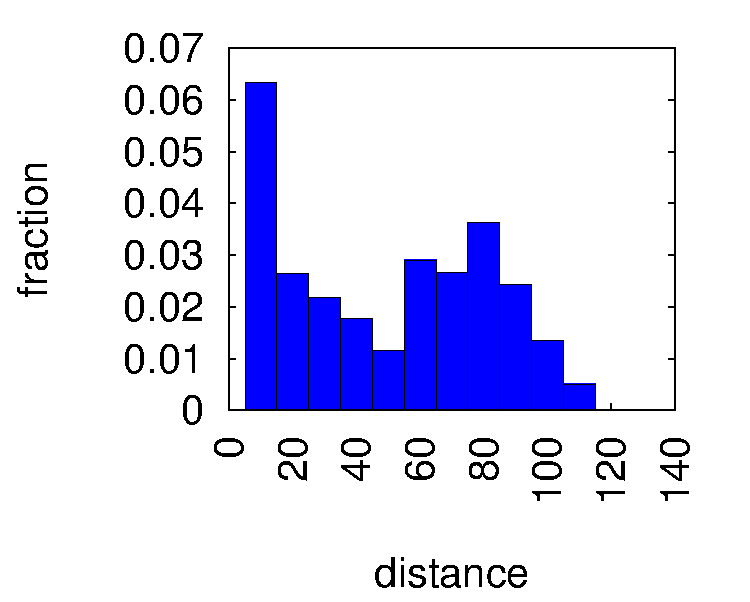
\includegraphics[width=0.3\textwidth]{/home/owodo/MINE/PROJECTS/GraSPI/GraSPI-2.0/examples/101x101/phi0_0.5/histograms/phasedataCH.0004.txtHistogramFullereneToCathode.pdf}} 
\parbox{0.33\textwidth}{\begin{scriptsize}Distance from Polymer Vertex to Anode\end{scriptsize}\newline
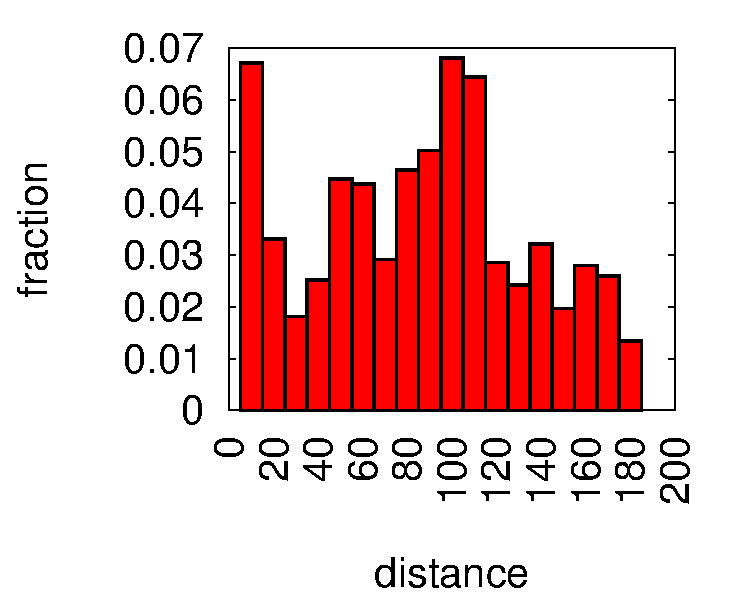
\includegraphics[width=0.3\textwidth]{/home/owodo/MINE/PROJECTS/GraSPI/GraSPI-2.0/examples/101x101/phi0_0.5/histograms/phasedataCH.0004.txtHistogramPolymerToAnode.pdf}}
\parbox{0.33\textwidth}{\begin{scriptsize}Distance from Polymer Vertex to Interface\end{scriptsize}\newline
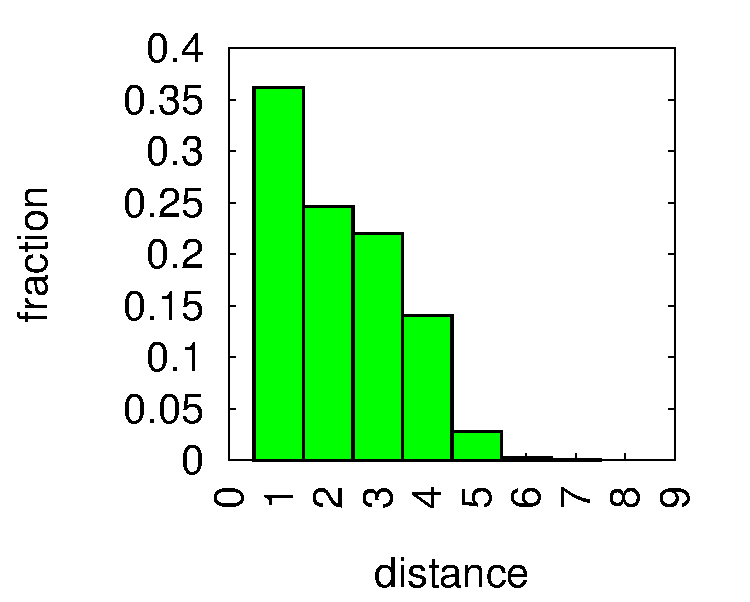
\includegraphics[width=0.3\textwidth]{/home/owodo/MINE/PROJECTS/GraSPI/GraSPI-2.0/examples/101x101/phi0_0.5/histograms/phasedataCH.0004.txtHistogramPolymerToInterface.pdf}} \newline
\parbox{0.49\textwidth}{\begin{scriptsize}Distance from Interface to Cathode via Fullerene vertices \end{scriptsize}\newline
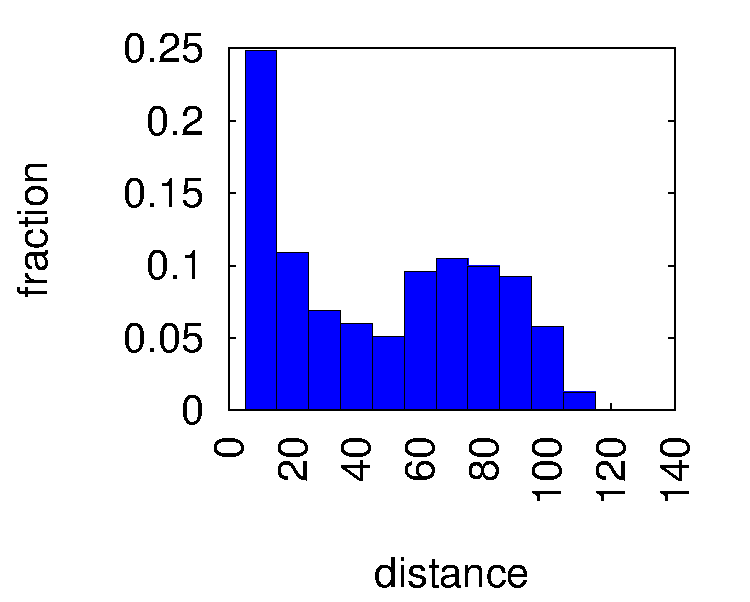
\includegraphics[width=0.33\textwidth]{/home/owodo/MINE/PROJECTS/GraSPI/GraSPI-2.0/examples/101x101/phi0_0.5/histograms/phasedataCH.0004.txtHistogramInterfaceToCathodeViaFullerene.pdf}}
\parbox{0.49\textwidth}{\begin{scriptsize}Distance from Interface to Anode via Polymer vertices \end{scriptsize}\newline
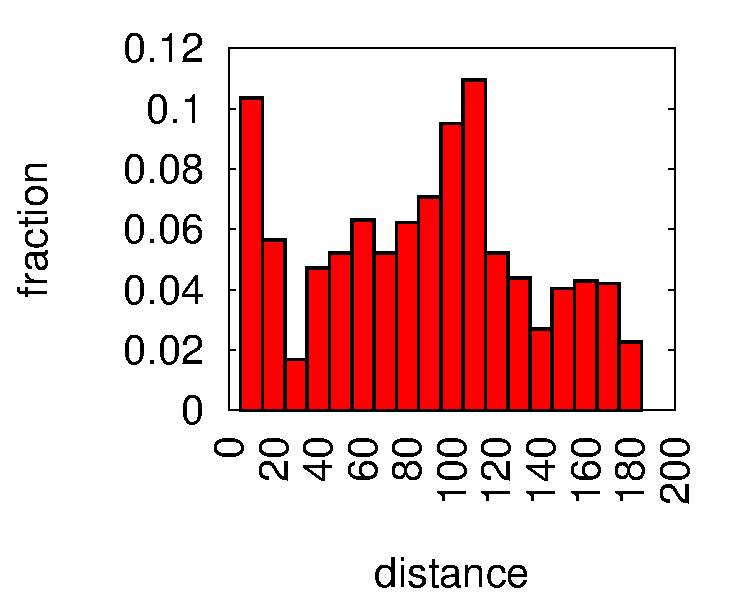
\includegraphics[width=0.33\textwidth]{/home/owodo/MINE/PROJECTS/GraSPI/GraSPI-2.0/examples/101x101/phi0_0.5/histograms/phasedataCH.0004.txtHistogramInterfaceToAnodeViaPolymer.pdf}}\newline
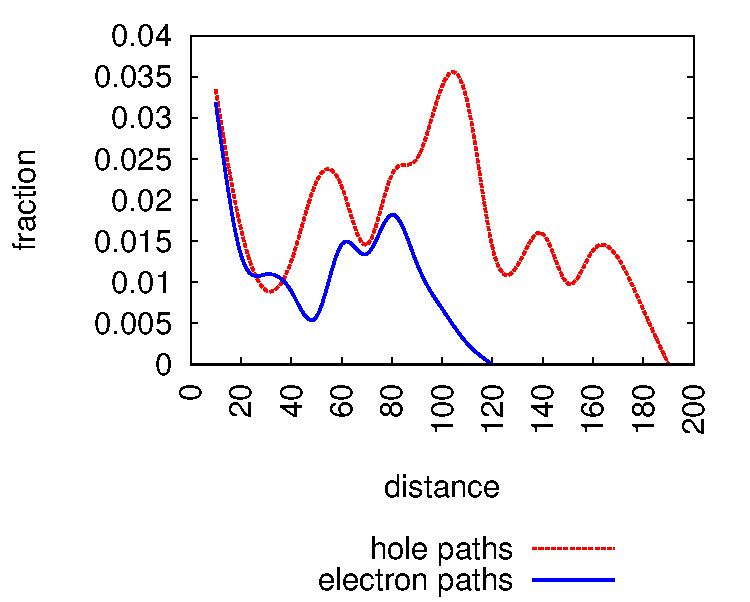
\includegraphics[width=0.33\textwidth]{/home/owodo/MINE/PROJECTS/GraSPI/GraSPI-2.0/examples/101x101/phi0_0.5/histograms/phasedataCH.0004.txtBothHistogramsUsefulDomains.pdf}
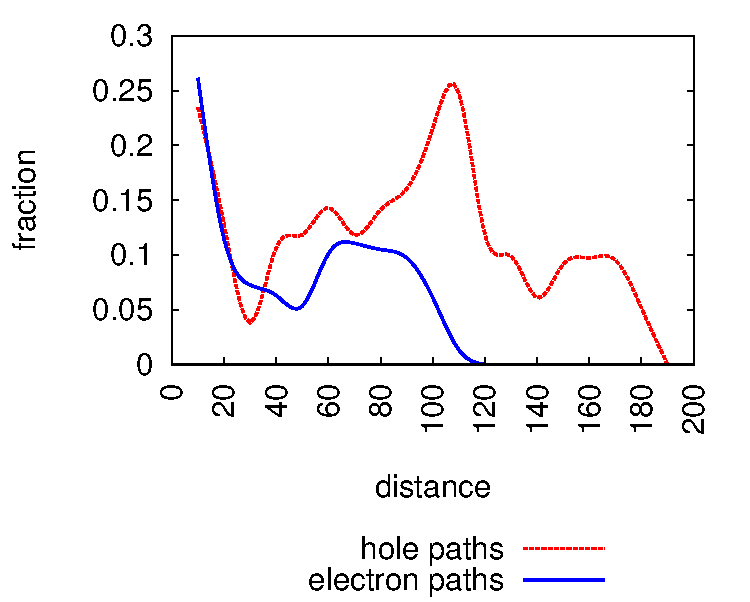
\includegraphics[width=0.33\textwidth]{/home/owodo/MINE/PROJECTS/GraSPI/GraSPI-2.0/examples/101x101/phi0_0.5/histograms/phasedataCH.0004.txtBothHistogramsUsefulInterface.pdf}
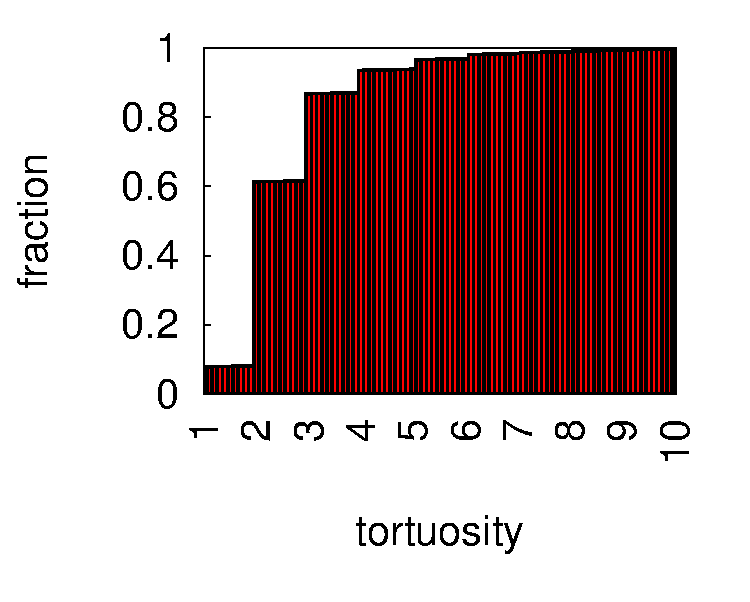
\includegraphics[width=0.33\textwidth]{/home/owodo/MINE/PROJECTS/GraSPI/GraSPI-2.0/examples/101x101/phi0_0.5/histograms/phasedataCH.0004.txtCumHistogramTortuosityPolymerToAnode.pdf}
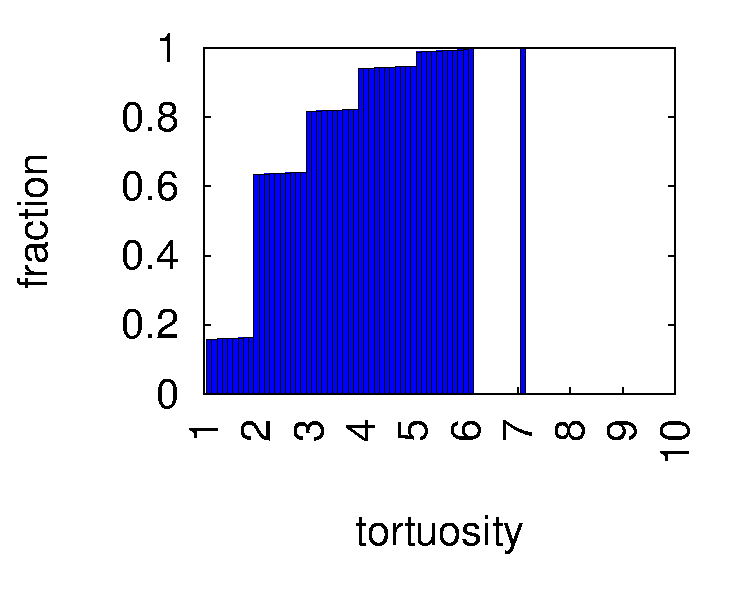
\includegraphics[width=0.33\textwidth]{/home/owodo/MINE/PROJECTS/GraSPI/GraSPI-2.0/examples/101x101/phi0_0.5/histograms/phasedataCH.0004.txtCumHistogramTortuosityFullereneToCathode.pdf}
\end{center}
\end{document}
